\documentclass[12pt,a4paper]{article}
\usepackage[top=1.5cm,bottom=1.5cm,left=2cm,right=1.5cm]{geometry}
\usepackage{fontspec}\setmainfont{TeX Gyre Termes}
\usepackage{amsmath,amssymb,tikz,tasks}
\setlength{\parindent}{0pt}
\newif\ifloigiai \loigiaitrue   % \loigiaifalse để in bản học sinh
\newenvironment{bai}[4]{\par\medskip\noindent\textbf{Bài #1. (#2 điểm)}\ }{\par}
% #1 số bài, #2 điểm, #3 mã dạng (vd B6-D2), #4 mã câu (vd TS10-D01-B6)
\newcommand{\y}[2]{\par\hspace*{1em}#1)~#2}             % ý a), b), c)
\newcommand{\loigiai}[1]{\ifloigiai\par\smallskip\noindent\textit{Lời giải.} #1\par\fi}
\newcommand{\diem}[1]{\ifloigiai\hfill\textbf{(#1đ)}\fi}  % điểm từng bước trong lời giải
\begin{document}
\begin{center}\textbf{ĐỀ ÔN TẬP TUYỂN SINH 10 – ĐỀ SỐ 42 – Mức: nâng cao}\\ Thời gian: 120 phút (không kể thời gian phát đề)\end{center}

\begin{bai}{1}{1,5}{B1-D2}{TS10-D42-B1}
Cho hàm số $y=-\dfrac{3}{2}x^2$ có đồ thị $(P)$.
\y{a}{Tìm toạ độ các điểm thuộc $(P)$ có tung độ bằng 2 lần hoành độ.}
\y{b}{Tìm toạ độ các điểm thuộc $(P)$ có tung độ bằng $-24$.}
\loigiai{
a) Gọi $N(x;y)\in(P)$ có tung độ bằng $2$ lần hoành độ, tức $y=2x$ và $y=-\dfrac{3}{2}x^2$. \diem{0,25}\\
Ta có phương trình $-\dfrac{3}{2}x^2=2x$, hay $x\left(-\dfrac{3}{2}x-2\right)=0$. Suy ra $x=0$ hoặc $x=-\dfrac{4}{3}$. \diem{0,25}\\
Với $x=0$ ta có $y=0$; với $x=-\dfrac{4}{3}$ ta có $y=2\cdot(-\dfrac{4}{3})=-\dfrac{8}{3}$. Vậy có hai điểm $O(0;0)$ và $(-\dfrac{4}{3};\,-\dfrac{8}{3})$. \diem{0,25}\\
b) Thay $y=-24$ vào $y=-\dfrac{3}{2}x^2$: $-\dfrac{3}{2}x^2=-24$, suy ra $x^2=16=4^2$. \diem{0,5}\\
Do đó $x=4$ hoặc $x=-4$. Vậy có hai điểm $(4;\,-24)$ và $(-4;\,-24)$. \diem{0,25}
\\\textit{Học sinh giải cách khác đúng vẫn cho điểm tối đa.}\\
\textbf{Đã kiểm chứng:} B1-D2: điểm (-4/3;-8/3) thoả y=2x; ±4 cho y=-24
}
\end{bai}

\begin{bai}{2}{1,0}{B2-D3}{TS10-D42-B2}
Cho phương trình $3x^2-5x-1=0$.
\y{a}{Chứng minh phương trình có hai nghiệm phân biệt $x_1$, $x_2$.}
\y{b}{Không giải phương trình, hãy tính $A=(x_1+2x_2)(2x_1+x_2)$.}
\loigiai{
a) Vì $a\cdot c=-3<0$ nên phương trình luôn có hai nghiệm phân biệt $x_1$, $x_2$. \diem{0,25} (Hoặc: $\Delta=37>0$.) \diem{0,25}\\[2pt]
b) Theo định lí Vi-ét: $x_1+x_2=\dfrac{5}{3}$ và $x_1x_2=-\dfrac{1}{3}$. \diem{0,25}\\
Ta có $A=2x_1^2+5x_1x_2+2x_2^2=2(x_1+x_2)^2+x_1x_2=2\cdot(\dfrac{5}{3})^2+(-\dfrac{1}{3})=\dfrac{47}{9}$. \diem{0,25}
\\\textit{Học sinh giải cách khác đúng vẫn cho điểm tối đa.}\\
\textbf{Đã kiểm chứng:} B2-D3: A= dfrac\{47\}\{9\} khớp nghiệm số
}
\end{bai}

\begin{bai}{3}{1,5}{B3-D2}{TS10-D42-B3}
Biểu đồ tròn dưới đây cho biết tỉ lệ các nhóm trong khảo sát về điểm kiểm tra Toán của 300 người (mỗi người chọn đúng một nhóm).
\begin{center}
\begin{tikzpicture}[scale=1,>=stealth,line cap=round]
\filldraw[fill=gray!10] (0,0)--(90.00:1.6) arc (90.00:-36.00:1.6)--cycle;
\node[font=\scriptsize,align=center,fill=white,inner sep=1pt] at (0.891,0.454) {4 điểm\\35\%};
\filldraw[fill=gray!30] (0,0)--(-36.00:1.6) arc (-36.00:-72.00:1.6)--cycle;
\node[font=\scriptsize,align=center,fill=white,inner sep=1pt] at (0.588,-0.809) {5 điểm\\10\%};
\filldraw[fill=gray!50] (0,0)--(-72.00:1.6) arc (-72.00:-180.00:1.6)--cycle;
\node[font=\scriptsize,align=center,fill=white,inner sep=1pt] at (-0.588,-0.809) {6 điểm\\30\%};
\filldraw[fill=gray!70] (0,0)--(-180.00:1.6) arc (-180.00:-252.00:1.6)--cycle;
\node[font=\scriptsize,align=center,fill=white,inner sep=1pt] at (-0.809,0.588) {7 điểm\\20\%};
\filldraw[fill=gray!20] (0,0)--(-252.00:1.6) arc (-252.00:-270.00:1.6)--cycle;
\node[font=\scriptsize,align=center,fill=white,inner sep=1pt] at (-0.156,0.988) {8 điểm\\5\%};
\end{tikzpicture}
\end{center}
\y{a}{Tính số người thuộc mỗi nhóm.}
\y{b}{Chọn ngẫu nhiên một người. Tính xác suất của biến cố $A$: "Người được chọn không thuộc nhóm 5 điểm".}
\y{c}{Chọn ngẫu nhiên một người. Tính xác suất của biến cố $B$: "Người được chọn thuộc nhóm 6 điểm hoặc nhóm 7 điểm".}
\loigiai{
a) nhóm "4 điểm": $35\%\cdot300=105$; nhóm "5 điểm": $10\%\cdot300=30$; nhóm "6 điểm": $30\%\cdot300=90$; nhóm "7 điểm": $20\%\cdot300=60$; nhóm "8 điểm": $5\%\cdot300=15$. \diem{0,5}\\
b) Số người không thuộc nhóm "5 điểm" là $300-30=270$. Vậy $P(A)=\dfrac{270}{300}=0{,}9$. \diem{0,5}\\
c) Số người thuộc nhóm "6 điểm" hoặc "7 điểm" là $90+60=150$. Vậy $P(B)=\dfrac{150}{300}=0{,}5$. \diem{0,5}
\\\textit{Học sinh giải cách khác đúng vẫn cho điểm tối đa.}\\
\textbf{Đã kiểm chứng:} B3-D2: tròn 300 người, tổng các nhóm = 300; P(A)=9/10; P(B)=1/2
}
\end{bai}

\begin{bai}{4}{1,0}{B4-D4}{TS10-D42-B4}
Phí vận chuyển một kiện hàng gồm 20\,000 đồng phí nhận hàng và 5\,000 đồng cho mỗi kilômét. Gọi $y$ (đồng) là phí vận chuyển quãng đường $x$ (km).
\y{a}{Lập công thức $y$ theo $x$.}
\y{b}{Tính phí vận chuyển quãng đường 10 km.}
\y{c}{Phí là 270\,000 đồng. Tính quãng đường vận chuyển.}
\loigiai{
a) $y=5\,000x+20\,000$. \diem{0,5}\\
b) $y=70\,000$ (đồng). \diem{0,25}\\
c) $x=\dfrac{270\,000-20\,000}{5\,000}=50$ (km). \diem{0,25}
\\\textit{Học sinh giải cách khác đúng vẫn cho điểm tối đa.}\\
\textbf{Đã kiểm chứng:} B4-D4: vận chuyển
}
\end{bai}

\begin{bai}{5}{1,0}{B5-D1}{TS10-D42-B5}
Một ly kem gồm phần vỏ bánh hình nón có bán kính đáy 5 cm, chiều cao 12 cm, đường sinh 13 cm, bên trên là một viên kem có dạng nửa hình cầu có cùng bán kính đáy với hình nón.
\y{a}{Tính thể tích của vật (hình nón và nửa hình cầu), làm tròn đến hàng phần mười của $\text{cm}^3$.}
\y{b}{Tính diện tích giấy bọc ngoài (gồm diện tích xung quanh hình nón và diện tích nửa mặt cầu), làm tròn đến hàng đơn vị của $\text{cm}^2$.}
Thể tích hình nón $V=\dfrac13\pi R^2h$, diện tích xung quanh hình nón $S=\pi Rl$ ($R$ là bán kính đáy, $h$ là chiều cao, $l$ là độ dài đường sinh). Thể tích hình cầu $V=\dfrac43\pi R^3$, diện tích mặt cầu $S=4\pi R^2$ ($R$ là bán kính). Lấy $\pi=3{,}14$.
\loigiai{
a) $V_{\text{nón}}=\dfrac13\pi R^2h=\dfrac13\cdot3{,}14\cdot5^2\cdot12=314{,}00$; $V_{\text{nửa cầu}}=\dfrac23\pi R^3=\dfrac23\cdot3{,}14\cdot5^3=261{,}67$ ($\text{cm}^3$). \diem{0,25}\\
Vậy $V\approx575{,}7\ \text{cm}^3$. \diem{0,25}\\[2pt]
b) $S_{\text{xq nón}}=\pi Rl=3{,}14\cdot5\cdot13=204{,}1$; $S_{\text{nửa cầu}}=2\pi R^2=2\cdot3{,}14\cdot5^2=157$ ($\text{cm}^2$). \diem{0,25}\\
Vậy $S\approx361\ \text{cm}^2$. \diem{0,25}
\\\textit{Học sinh giải cách khác đúng vẫn cho điểm tối đa.}\\
\textbf{Đã kiểm chứng:} B5-D1: nón+nửa cầu r=5 h=12: V=575.667, S=361.100
}
\end{bai}

\begin{bai}{6}{1,0}{B6-D7}{TS10-D42-B6}
Cô giáo chia một số kẹo cho học sinh trong lớp. Nếu mỗi bạn nhận $5$ cái thì còn thừa $10$ cái; nếu mỗi bạn nhận $6$ cái thì thiếu $10$ cái. Gọi $x$ là số học sinh, $y$ là số cái kẹo.
\y{a}{Lập hệ phương trình theo $x$, $y$.}
\y{b}{Tính số học sinh và số kẹo.}
\loigiai{
a) $y=5x+10$ $(1)$ và $y=6x-10$ $(2)$. \diem{0,5}\\
b) Trừ $(2)$ cho $(1)$ vế theo vế: $0=x-20$, suy ra $x=20$; thay vào $(1)$ được $y=110$. Vậy lớp có $20$ học sinh và $110$ cái kẹo. \diem{0,5}
\\\textit{Học sinh giải cách khác đúng vẫn cho điểm tối đa.}\\
\textbf{Đã kiểm chứng:} B6-D7: chia kẹo x=20,y=110
}
\end{bai}

\begin{bai}{7}{3,0}{B7-C6/c-TINH}{TS10-D42-B7}
Cho tam giác $ABC$ vuông tại $A$. Đường tròn $(O)$ đường kính $AB$ ($O$ là trung điểm của $AB$, bán kính $R$) cắt $BC$ tại điểm thứ hai $D$. Tiếp tuyến tại $D$ của $(O)$ cắt $AC$ tại $E$.
\y{a}{Chứng minh $AD\perp BC$ và $EA=ED$.}
\y{b}{Chứng minh $E$ là trung điểm của $AC$.}
\y{c}{Cho biết $\widehat{ABC}=60^\circ$. Tính diện tích tứ giác $ABDE$ theo $R$.}
\loigiai{
\begin{center}
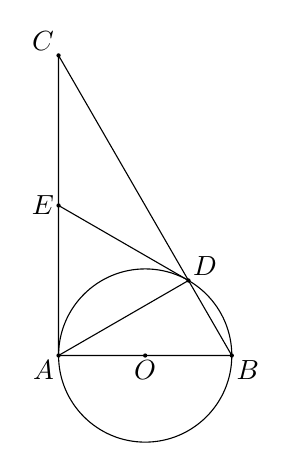
\begin{tikzpicture}[scale=1.1,>=stealth,line cap=round]
\coordinate (A) at (-1.0000,0.0000);
\coordinate (B) at (1.0000,0.0000);
\coordinate (C) at (-1.0000,3.4641);
\coordinate (D) at (0.5000,0.8660);
\coordinate (E) at (-1.0000,1.7321);
\coordinate (O) at (0.0000,0.0000);
\draw (O) circle (1);
\draw (A)--(B)--(C)--cycle;
\draw (A)--(D); \draw (E)--(D);
\fill (A) circle (0.7pt);
\fill (B) circle (0.7pt);
\fill (C) circle (0.7pt);
\fill (D) circle (0.7pt);
\fill (E) circle (0.7pt);
\fill (O) circle (0.7pt);
\node[below left,inner sep=1.5pt] at (A) {$A$};
\node[below right,inner sep=1.5pt] at (B) {$B$};
\node[above left,inner sep=1.5pt] at (C) {$C$};
\node[above right,inner sep=1.5pt] at (D) {$D$};
\node[left,inner sep=1.5pt] at (E) {$E$};
\node[below,inner sep=1.5pt] at (O) {$O$};
\end{tikzpicture}
\end{center}
a) Vì $D$ thuộc đường tròn đường kính $AB$ nên $\widehat{ADB}=90^\circ$, tức $AD\perp BC$. \diem{0,5}\\
Vì $\widehat{BAC}=90^\circ$ nên $EA$ là tiếp tuyến của $(O)$ tại $A$; $ED$ là tiếp tuyến tại $D$. Hai tiếp tuyến cắt nhau tại $E$ nên $EA=ED$. \diem{0,5}\\[2pt]
b) Vì $EA=ED$ nên $\widehat{EAD}=\widehat{EDA}$. \diem{0,25}\\
Trong tam giác $ADC$ vuông tại $D$: $\widehat{EAD}+\widehat{ECD}=90^\circ$ và $\widehat{EDA}+\widehat{EDC}=90^\circ$. \diem{0,25}\\
Suy ra $\widehat{EDC}=\widehat{ECD}$, nên $ED=EC$. \diem{0,25}\\
Mà $EA=ED$ nên $EA=EC$, tức $E$ là trung điểm của $AC$. \diem{0,25}\\[2pt]
c) Tam giác $ABC$ vuông tại $A$ có $AB=2R$, $\widehat{ABC}=60^\circ$ nên $AC=AB\tan60^\circ=2 \sqrt{3} R$ và $BC=\dfrac{AB}{\cos60^\circ}=4 R$. Theo hệ thức lượng trong tam giác vuông $ABC$ (đường cao $AD$): $AD=\dfrac{AB\cdot AC}{BC}=\sqrt{3} R$, $BD=\dfrac{AB^2}{BC}=R$, $DC=\dfrac{AC^2}{BC}=3 R$. \diem{0,5}\\
Đường chéo $AD$ chia tứ giác $ABDE$ thành hai tam giác $ABD$ và $ADE$. \diem{0,25}\\
$S_{ABD}=\dfrac12\,AD\cdot BD=\dfrac{\sqrt{3} R^{2}}{2}$ và $S_{ADE}=\dfrac14\,AD\cdot DC=\dfrac{3 \sqrt{3} R^{2}}{4}$ (do $E$ là trung điểm $AC$). Vậy $S_{ABDE}=\dfrac{5 \sqrt{3} R^{2}}{4}$. \diem{0,25}
\\\textit{Học sinh giải cách khác đúng vẫn cho điểm tối đa.}\\
\textbf{Đã kiểm chứng:} C6/T6: toạ độ R=1, $\angle$B=60$^\circ$, số liệu c khớp
}
\end{bai}
\ifloigiai
\begin{samepage}\bigskip\noindent\textbf{Bảng tóm tắt kiểm chứng.}\par\smallskip
{\small\begin{tabular}{|c|c|c|l|}
\hline Đề số & Mức & Mã dạng & Đã kiểm chứng\\\hline
42 & nâng cao & B1-D2 & Có (Python) \\\hline
42 & nâng cao & B2-D3 & Có (Python) \\\hline
42 & nâng cao & B3-D2 & Có (Python) \\\hline
42 & nâng cao & B4-D4 & Có (Python) \\\hline
42 & nâng cao & B5-D1 & Có (Python) \\\hline
42 & nâng cao & B6-D7 & Có (Python) \\\hline
42 & nâng cao & B7-C6/c-TINH & Có (Python) \\\hline
\end{tabular}}
\end{samepage}
\fi
\end{document}
